\chapter{Introduction}
\label{cha:introduction}

% The following sections suggest an outline proposal for a first chapter of a bachelor/ master thesis written
% by Cooperation \& Management (C\&M) at Karlsruhe Institute of Technology (KIT).  

\section{Introduction to the Topic Area}
% If the work is based on a concrete project scenario, this project scenario should already be introduced
% in this section at a high level of abstraction.


\section{Research Questions}
% The first research question should be superior to the following questions ''2 to n'' 
% and should be dealt with in the first content chapter which is Chapter 4.

% The second research question concerns the concrete software system which serves as a (first part of a)
% demonstrator for the overall research question. This software system will be developed in cooperation with
%  the project team (JuniorStudents) which is co-supervised by the author (SeniorStudent) of this thesis.
% Chapter 5 (Technical Foundation) introduces the existing preliminary work which particularly includes the already
% existing artifacts relevant for the software system to be developed. Chapter 6 (First Solution) describes the
% structured development approach of the software system (in the case of a microservice-based application,
% this is C\&M's microservice engineering approach).

% Research questions 3 to n should then be addressed in the following chapters.
% These research questions should be formulated in detail only AFTER clear answers to the second research question have
% been worked out since these results have a strong influence on the further alignment of the thesis.

\section{Description of the Demonstrator}
% The demonstrator should clarify the research questions introduced in the previous section on an appropriate conceptual level.
% The demonstrator introduces a practical example and shows a solution. In its first draft,
% it corresponds to the software system which is developed in cooperation with the co-supervised project team (JuniorStudents).

\section{Thesis Structure}
% \label{sec:gliederung}
% This chapter illustrates the structure of the work in the form of the chapter structure.
% The following chapter structure is recommended:

% \subsection*{Chapter 2: Foundations}
% This chapter contains information necessary for a basic understanding of the thesis.
% The information is presented as ''value-free'' as possible.

% \subsection*{Chapter 3: State of the Art}
% The results of the Top Literature are an essential part of this chapter. The structure described in the introduction can be recalled here.

% In contrast to Chapter 2, the contents of this chapter are presented in an argumentative and evaluative form.

% \subsection*{Chapter 4: First Content Chapter}
% Chapters 4 to 4+n are the conceptual contribution chapters of the work in which the achieved results are described.

% \subsubsection*{Chapter 5: ...}

% \subsubsection*{Chapter 6: ...}

% \subsection*{Chapter 5+n: Project Team Work}
% The second last chapter contains the results of the project team work.
% The chapter also describes events (e.g. Coding Day, visits to institutes) in which the person working on this thesis has participated.

\section{Content-related Overview}
% The overview should describe the most important topic dependencies by means of an illustration.

\section{Further Information}
% \textit{This section provides various notes on language conventions, formatting, or other technical aspects.
% Therefore, this section must be removed before completing the Bachelor's/Master's thesis.}

% \subsection{Inserting PowerPoint Figures}
% Images are exclusively created with PowerPoint in the image document which should contain all figures in the order of their
% appearance in the thesis document. The title of the slide in the thesis figures file document should correspond to the title of
% the figure in the thesis document. The thesis figures file is saved as .png in the Overleaf folder ``figures''.

% Inserting and referencing the figure is done by a reference: Figure \ref{fig:the_fig_fil_pro}.

% \begin{figure}[h]
% 	\centering
% 	
\includegraphics[width=0.8\textwidth]{figures/the_fig_fil_pro.png}
% 	\caption{Thesis Figures File Process}
% 	\label{fig:the_fig_fil_pro}
% \end{figure}

% The steps of the process described in Figure \ref{fig:the_fig_fil_pro} should be carried out by each JuniorStudent
% and SeniorStudent when creating the initial version of the thesis document.

% \subsection{Inserting UML Diagrams}
% UML diagrams are exclusively created with the tool UMLet. The UMLet files are to be stored in the subfolder ``6.UMLet\_Sources''.
% The UMLet diagram is inserted in the format .png in the thesis figures file. The UMLet diagram illustrated in Figure \ref{fig:exa_sys_arc}
% is taken from the WASA lecture.

% \begin{figure}[ht]
% 	\centering
% 	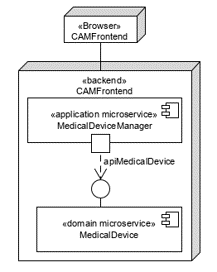
\includegraphics[width=0.4\textwidth]{figures/exa_sys_arc}
% 	\caption{Example of a SystemPlusSoftware Architecture}
% 	\label{fig:exa_sys_arc}
% \end{figure}

% The naming convention of the UMLet file is <figure\_number>.<tite\_of\_the\_figure> as can be easily understood when taking
% a closer look to the folder ``6.UMLet\_Sources'' in which the example diagram shown in Figure \ref{fig:exa_sys_arc} is stored.

% \subsection{Citations}
% \label{subsec:citations}
% Citations can be included in the thesis in the following way:

% \begin{quote}
% \textit{``A microservice is a cohesive, independent process interacting via messages''}
% \end{quote}
% \begin{quote}
% \textit{``fictive book quote.'', \cite[P.~99]{Be02}}
% \end{quote}

% \subsection{Writing Cucumber Features in LaTeX}
% Features are included in the LaTeX code as a special listing and referenced in the text using the feature \ref{lis:example} command.

% \vspace{0.5cm}
% \begin{lstlisting}[caption = {Example for Development Artifacts in the Thesis}, label = {lis:example}, style = kit-cm, language=] 
% First line of the development artifact
% Second line of the development artifact
% \end{lstlisting}

% \subsection{Inserting Tables}
% Table \ref{tab:example_table} shows an simple example for inserting a table in LaTeX.
% \begin{table}[H] 
%Hint: The [H] is part of the packet float. It stands for ``Here'' which means that the table is placed where it is defined.
% 	\centering
% 	\begin{tabular}{ | l | p{7cm} | }
% 		\hline
% 		\textbf{Heading} & \textbf{Further Heading} \\
% 		\hline
% 		 Entry & Example of an entry \\
% 		\hline
% 		 Entry & Example of a further entry \\
% 	 	\hline
% 	\end{tabular}
% 	\caption{Example of a Table}
% 	\label{tab:example_table}
% \end{table}

% \subsection{Linguistic Conventions in the Context of the C\&M Software Development Process}
% All artifacts created during the C\&M software development process are written in English.
% This also applies to the features created in the analysis phase, since it is assumed that the user of a software system
% developed by C\&M is an English speaker. American English is used throughout the thesis.

% An important quality aspect to be considered in software development is the consistent spelling of the introduced terms during development.
% Two levels must be distinguished here: The level of ("natural", English) language and the level of (formal, development-related) artifacts.
% An example of a term at the language level is "Todo List Management".
% As a C\&M convention that terms are written on the artifact level in the so-called CamelCase notation, in this example "TodoListManagement".